% Compilar con: xelatex informe_gradio.tex (dos veces)
\documentclass[11pt,letterpaper]{article}

\usepackage[spanish,es-nodecimaldot]{babel}
\usepackage{fontspec}
\setmainfont{Arial}
\setsansfont{Arial}
\setmonofont{Consolas}
\usepackage[letterpaper,margin=2.15cm,headheight=16pt]{geometry}
\usepackage{xcolor}
\usepackage{graphicx}
\usepackage{booktabs}
\usepackage{tabularx}
\usepackage{longtable}
\usepackage{array}
\usepackage{amsmath}
\usepackage{enumitem}
\usepackage{fancyhdr}
\usepackage{hyperref}
\usepackage{fancyvrb}
\usepackage{tcolorbox}
\usepackage{tikz}
\usetikzlibrary{arrows.meta,positioning,calc,shapes.geometric}
\usepackage{float}
\usepackage{multicol}

\definecolor{UVGBlue}{HTML}{17365D}
\definecolor{Ink}{HTML}{111827}
\definecolor{Muted}{HTML}{5F6B7A}
\definecolor{Paper}{HTML}{F3F5F8}
\definecolor{GradioViolet}{HTML}{6657EF}
\definecolor{GradioOrange}{HTML}{F5743C}
\definecolor{Success}{HTML}{168B6A}
\definecolor{Rule}{HTML}{D4D9E1}

\hypersetup{
  colorlinks=true,
  linkcolor=UVGBlue,
  urlcolor=GradioViolet,
  citecolor=GradioOrange,
  pdftitle={Gradio para dashboards interactivos},
  pdfauthor={Pablo Daniel Barillas Moreno y Carlos Aldana}
}

\pagestyle{fancy}
\fancyhf{}
\fancyhead[L]{\small\color{Muted}CC3084 - Data Science}
\fancyhead[R]{\small\color{Muted}Grupo 6 - Sección 10}
\fancyfoot[L]{\small\color{Muted}Universidad del Valle de Guatemala}
\fancyfoot[R]{\small\color{Muted}\thepage}
\renewcommand{\headrulewidth}{0.4pt}
\renewcommand{\footrulewidth}{0pt}

\makeatletter
\renewcommand\section{\@startsection{section}{1}{0pt}{2.1ex plus .4ex}{0.8ex}{\color{UVGBlue}\Large\bfseries}}
\renewcommand\subsection{\@startsection{subsection}{2}{0pt}{1.5ex plus .3ex}{0.55ex}{\color{Ink}\large\bfseries}}
\makeatother

\setlength{\parindent}{0pt}
\setlength{\parskip}{0.62em}
\setlist[itemize]{leftmargin=1.4em,itemsep=0.3em,topsep=0.35em}
\setlist[enumerate]{leftmargin=1.6em,itemsep=0.35em,topsep=0.35em}
\renewcommand{\arraystretch}{1.28}

\newtcolorbox{keybox}[1][]{
  colback=Paper,
  colframe=GradioViolet,
  boxrule=0.8pt,
  arc=2mm,
  left=4mm,right=4mm,top=3mm,bottom=3mm,
  #1
}

\newtcolorbox{warningbox}[1][]{
  colback=GradioOrange!7,
  colframe=GradioOrange,
  boxrule=0.8pt,
  arc=2mm,
  left=4mm,right=4mm,top=3mm,bottom=3mm,
  #1
}

\DefineVerbatimEnvironment{codeblock}{Verbatim}{
  fontsize=\small,
  frame=single,
  framesep=3mm,
  rulecolor=\color{GradioViolet},
  numbers=left,
  numbersep=7pt,
  xleftmargin=7mm
}

\newcommand{\metric}[2]{%
  \begin{minipage}[t]{0.23\textwidth}
  \color{GradioViolet}\bfseries\fontsize{24}{26}\selectfont #1\\[-2pt]
  \color{Muted}\normalsize #2
  \end{minipage}
}

\begin{document}

\begin{titlepage}
\begin{tikzpicture}[remember picture,overlay]
  \fill[UVGBlue] (current page.north west) rectangle ([xshift=2.2cm]current page.south west);
  \fill[GradioViolet] ([xshift=2.2cm]current page.north west) rectangle ([xshift=2.38cm]current page.south west);
  \draw[GradioViolet,line width=17pt] ([xshift=-3.1cm,yshift=-3.0cm]current page.north east) circle (1.5cm);
  \fill[GradioOrange] ([xshift=-3.1cm,yshift=-3.0cm]current page.north east) circle (0.55cm);
\end{tikzpicture}

\vspace*{1.0cm}
\hspace*{1.65cm}
\begin{minipage}{0.80\textwidth}
\raggedright
{\color{GradioOrange}\bfseries\large CC3084 \textperiodcentered\ Data Science \textperiodcentered\ Sección 10 \textperiodcentered\ Grupo 6}

\vspace{1.3cm}
{\color{UVGBlue}\bfseries\fontsize{37}{41}\selectfont Gradio para\\dashboards interactivos\par}

\vspace{0.5cm}
{\color{Muted}\Large Investigación, comparación, arquitectura e implementación de un observatorio comercial reproducible}

\vspace{1.5cm}
\begin{keybox}
\textbf{Universidad del Valle de Guatemala}\\
Segundo semestre de 2026
\end{keybox}

\vspace{1.2cm}
{\large\bfseries Pablo Daniel Barillas Moreno}\hfill {\large Carné No. 222193}\\[0.35cm]
{\large\bfseries Carlos Aldana}\hfill {\large Carné No. 23394}

\vfill
{\color{Muted}Guatemala, octubre de 2026}
\end{minipage}
\end{titlepage}

\tableofcontents
\newpage

\section{Resumen ejecutivo}

Gradio es un paquete de código abierto orientado a convertir funciones, modelos y servicios de Python en aplicaciones web interactivas. Su principal ventaja consiste en reducir la distancia entre una pieza de lógica computacional y una experiencia que puede ser utilizada por una persona no especializada. El artículo original presentó esta idea como una respuesta al problema de accesibilidad y retroalimentación en proyectos de aprendizaje automático \cite{abid2019gradio}.

Este informe estudia Gradio como herramienta principal para dashboards interactivos, lo compara con Streamlit, Dash, Panel y Shiny, explica su modelo de programación y examina aspectos que suelen omitirse en un ejemplo básico: estado, eventos, colas, concurrencia, publicación, seguridad de archivos y criterios de uso en producción. Como aplicación práctica, se desarrolló un observatorio comercial con 576 registros sintéticos, filtros coordinados, cinco indicadores, cuatro visualizaciones, hallazgos automáticos y exportación CSV.

\begin{keybox}[title=Resultado central]
Gradio resulta especialmente conveniente cuando el valor principal ya existe como función, modelo o pipeline de Python y se necesita una interfaz demostrable con rapidez. No sustituye automáticamente un sistema de inteligencia de negocios ni un frontend empresarial hecho a medida; su idoneidad depende de los requisitos de gobierno, diseño, escala y operación.
\end{keybox}

\section{Objetivos y alcance}

\subsection{Objetivo general}

Investigar y demostrar el uso de Gradio para construir dashboards interactivos, identificando su arquitectura, ecosistema, fortalezas, limitaciones y posibilidades de despliegue.

\subsection{Objetivos específicos}

\begin{itemize}
  \item Definir qué distingue a un dashboard interactivo de un reporte estático.
  \item Explicar el papel de \texttt{Interface}, \texttt{Blocks}, componentes y eventos.
  \item Comparar Gradio con alternativas relevantes del ecosistema de datos.
  \item Construir una aplicación más cercana a un caso analítico real que a un simple ``Hola mundo''.
  \item Documentar instalación, pruebas, publicación, rendimiento y seguridad.
  \item Producir artefactos reproducibles: código Python, presentación HTML e informe PDF.
\end{itemize}

El proyecto utiliza datos sintéticos; no pretende realizar inferencias sobre una empresa real. Las conclusiones técnicas se apoyan en documentación oficial consultada en octubre de 2026 y en pruebas locales con Gradio 6.30.0.

\section{Dashboards interactivos}

Un dashboard interactivo reúne indicadores, tablas y visualizaciones en una interfaz que responde a acciones del usuario. La interacción permite formular preguntas sucesivas: seleccionar un periodo, aislar una región, comparar categorías, cambiar la métrica o descargar el subconjunto resultante. Por ello, el dashboard no es solamente una colección de gráficas; es un mecanismo de exploración y comunicación.

\begin{center}
\begin{tikzpicture}[
  node distance=1.1cm,
  box/.style={draw=Rule,rounded corners=2mm,fill=Paper,minimum width=3.05cm,minimum height=1.25cm,align=center,font=\bfseries},
  arrow/.style={-{Latex[length=3mm]},thick,color=GradioOrange}
]
  \node[box] (observe) {Observar\\\small KPIs y patrones};
  \node[box,right=of observe] (ask) {Preguntar\\\small filtros y controles};
  \node[box,right=of ask] (compare) {Comparar\\\small segmentos y metas};
  \node[box,right=of compare] (act) {Actuar\\\small comunicar o exportar};
  \draw[arrow] (observe) -- (ask);
  \draw[arrow] (ask) -- (compare);
  \draw[arrow] (compare) -- (act);
\end{tikzpicture}
\end{center}

Una solución útil debe equilibrar cinco dimensiones: claridad visual, capacidad analítica, tiempo de desarrollo, facilidad de publicación y sostenibilidad operativa. Una herramienta excelente para prototipos puede no ser la mejor elección para un portal corporativo con cientos de usuarios, identidad visual estricta y controles avanzados de acceso.

\section{Qué es Gradio}

Gradio es un paquete abierto de Python que genera interfaces web para funciones, modelos de aprendizaje automático, APIs y flujos arbitrarios. El inicio rápido oficial enfatiza que una aplicación básica no requiere conocimientos de JavaScript, CSS ni alojamiento web para comenzar \cite{gradioquickstart}. El proyecto se distribuye bajo licencia Apache 2.0 y su desarrollo ocurre públicamente en GitHub \cite{gradiogithub}.

\subsection{Origen y propósito}

Abid et al. propusieron Gradio en 2019 para facilitar que especialistas de dominio pudieran probar modelos y aportar retroalimentación sin reproducir el entorno técnico del investigador \cite{abid2019gradio}. Ese propósito explica varias decisiones de diseño actuales:

\begin{itemize}
  \item declarar entradas y salidas de forma explícita;
  \item soportar texto, imágenes, audio, video, archivos, tablas y gráficas;
  \item compartir una aplicación mediante una URL;
  \item ejecutar la lógica en Python y presentar el resultado en el navegador;
  \item ofrecer clientes programáticos además de la interfaz visual.
\end{itemize}

\subsection{Lenguajes y ecosistema}

Python es el lenguaje principal de autoría. El paquete \texttt{gradio\_client} permite consumir aplicaciones desde Python, mientras que \texttt{@gradio/client} habilita consumo desde JavaScript o TypeScript. Una aplicación alojada puede actuar simultáneamente como interfaz humana y como endpoint programático. Hugging Face Spaces ofrece integración directa para alojar demos Gradio en repositorios versionados \cite{hfspaces}.

\section{Modelo de programación}

\subsection{Tres niveles principales}

\begin{tabularx}{\textwidth}{>{\bfseries}p{2.8cm} X X}
\toprule
Abstracción & Propósito & Uso apropiado \\
\midrule
\texttt{Interface} & Envuelve una función con componentes de entrada y salida. & Demos pequeñas, prototipos y validación rápida. \\
\texttt{Blocks} & Controla layout, eventos y flujos entre múltiples componentes. & Dashboards, herramientas con pestañas y aplicaciones coordinadas. \\
\texttt{ChatInterface} & Implementa el patrón conversacional con historial y streaming. & Asistentes, chatbots y experiencias multimodales. \\
\bottomrule
\end{tabularx}

La documentación describe \texttt{Blocks} como la API de menor nivel que ofrece mayor control sobre layout, eventos y flujos de datos \cite{gradioblocks}. Los componentes funcionan como nodos visibles; los eventos conectan esos nodos con funciones de Python.

\subsection{Ejemplo mínimo}

\textbf{Interfaz mínima con Gradio}
\begin{codeblock}
import gradio as gr

def saludar(nombre, intensidad):
    return f"Hola, {nombre}" + "!" * int(intensidad)

demo = gr.Interface(
    fn=saludar,
    inputs=[gr.Textbox(label="Nombre"), gr.Slider(1, 5, step=1)],
    outputs=gr.Textbox(label="Resultado"),
)

demo.launch()
\end{codeblock}

El patrón consta de cuatro pasos: escribir una función, declarar componentes, conectarlos y lanzar el servidor. En desarrollo, \texttt{gradio app.py} habilita recarga automática; \texttt{python app.py} inicia la aplicación normalmente \cite{gradioquickstart}.

\section{Arquitectura y flujo de datos}

\begin{figure}[H]
\centering
\begin{tikzpicture}[
  node distance=1.25cm,
  layer/.style={draw=UVGBlue,rounded corners=2mm,fill=Paper,minimum width=3.1cm,minimum height=1.35cm,align=center},
  arrow/.style={-{Latex[length=3mm]},line width=1.2pt,color=GradioViolet}
]
  \node[layer] (user) {Usuario\\\small navegador};
  \node[layer,right=of user] (component) {Componentes\\\small entrada y salida};
  \node[layer,right=of component] (event) {Evento Gradio\\\small cola y validación};
  \node[layer,right=of event] (python) {Función Python\\\small datos, API o modelo};
  \draw[arrow] (user) -- node[above,sloped,font=\scriptsize]{acción} (component);
  \draw[arrow] (component) -- node[above,sloped,font=\scriptsize]{valores} (event);
  \draw[arrow] (event) -- node[above,sloped,font=\scriptsize]{llamada} (python);
  \draw[arrow,bend right=35] (python.south) to node[below,font=\scriptsize]{resultado} (component.south);
\end{tikzpicture}
\caption{Flujo simplificado de una interacción en Gradio.}
\end{figure}

La función recibe valores ya serializados por los componentes y devuelve resultados que Gradio transforma para el navegador. Este contrato facilita reemplazar una función simple por una operación más compleja sin rediseñar toda la interfaz.

\subsection{Estado}

La documentación distingue tres alcances \cite{gradiostate}:

\begin{itemize}
  \item \textbf{Global}: compartido por todos los usuarios mientras el proceso está activo.
  \item \textbf{Sesión}: aislado por usuario durante la sesión mediante \texttt{gr.State}.
  \item \textbf{Navegador}: persistente en almacenamiento local mediante \texttt{gr.BrowserState}.
\end{itemize}

Elegir el alcance incorrecto puede mezclar información entre usuarios o perder preferencias al recargar. El estado global es conveniente para recursos inmutables, como un modelo cargado una vez, pero no para datos privados de una sesión.

\subsection{Colas y concurrencia}

Cada listener dispone de una cola. El parámetro \texttt{concurrency\_limit} controla cuántas ejecuciones simultáneas admite un evento; los listeners también pueden compartir una cola mediante un identificador común \cite{gradioqueue}. Esto es relevante cuando una operación consume GPU, memoria significativa o una API limitada. Aumentar concurrencia sin medir recursos puede elevar la latencia o producir errores por agotamiento de memoria.

\section{Comparación con otras herramientas}

\begin{longtable}{>{\bfseries}p{2.35cm} p{2.35cm} p{4.45cm} p{5.05cm}}
\toprule
Herramienta & Lenguaje & Fortalezas & Consideraciones \\
\midrule
\endhead
Gradio & Python; clientes Python y JS/TS & Interfaces rápidas para modelos, funciones, multimedia y APIs; publicación sencilla; API automática. & Menor control que un frontend a medida; debe evaluarse seguridad, concurrencia y operación. \\
Streamlit & Python & Modelo de ejecución accesible, ecosistema amplio para aplicaciones de datos y prototipos. & El patrón de reejecución requiere comprender estado y caché en aplicaciones grandes \cite{streamlitdocs}. \\
Dash & Python & Control explícito mediante callbacks, integración natural con Plotly y aplicaciones analíticas. & Puede requerir más estructura y código para prototipos pequeños \cite{dashdocs}. \\
Panel & Python & Integración profunda con PyData, HoloViz, notebooks y múltiples librerías de visualización. & Flexibilidad amplia implica más decisiones arquitectónicas \cite{paneldocs}. \\
Shiny & R y Python & Modelo reactivo maduro, modularidad y fuerte tradición estadística. & La elección suele depender del ecosistema R/Python y de la plataforma de publicación \cite{shinydocs}. \\
\bottomrule
\end{longtable}

\begin{keybox}[title=Criterio práctico]
Si el núcleo es un modelo o una función Python que debe demostrarse pronto, Gradio suele reducir el tiempo hasta la primera versión. Si el núcleo es un producto web con navegación compleja, diseño altamente personalizado o gobierno empresarial, conviene comparar una arquitectura web completa o herramientas analíticas más especializadas.
\end{keybox}

\section{Aplicación desarrollada por el grupo}

El proyecto implementa un \textit{observatorio comercial} con datos sintéticos de 2026. El dataset se genera de manera determinista para asegurar que la exposición y las pruebas produzcan siempre los mismos resultados.

\begin{center}
\metric{576}{observaciones}\hfill
\metric{12}{meses}\hfill
\metric{4}{regiones}\hfill
\metric{4 x 3}{categorías y canales}
\end{center}

\subsection{Variables y funcionalidades}

Cada observación contiene fecha, región, categoría, canal, ventas, costo, margen bruto, unidades, pedidos y satisfacción. La interfaz incorpora:

\begin{itemize}
  \item filtros multiselección por región, categoría y canal;
  \item mes inicial, mes final y meta mensual configurable;
  \item selección de métrica y tipo de visualización;
  \item cinco KPIs: ventas, crecimiento, margen, ticket y cumplimiento;
  \item tendencia mensual, mezcla por categoría, rendimiento regional y mapa de calor;
  \item hallazgos narrativos generados desde el subconjunto filtrado;
  \item tabla detallada y descarga CSV;
  \item restablecimiento de estado y cola con límite de concurrencia.
\end{itemize}

\begin{figure}[H]
\centering
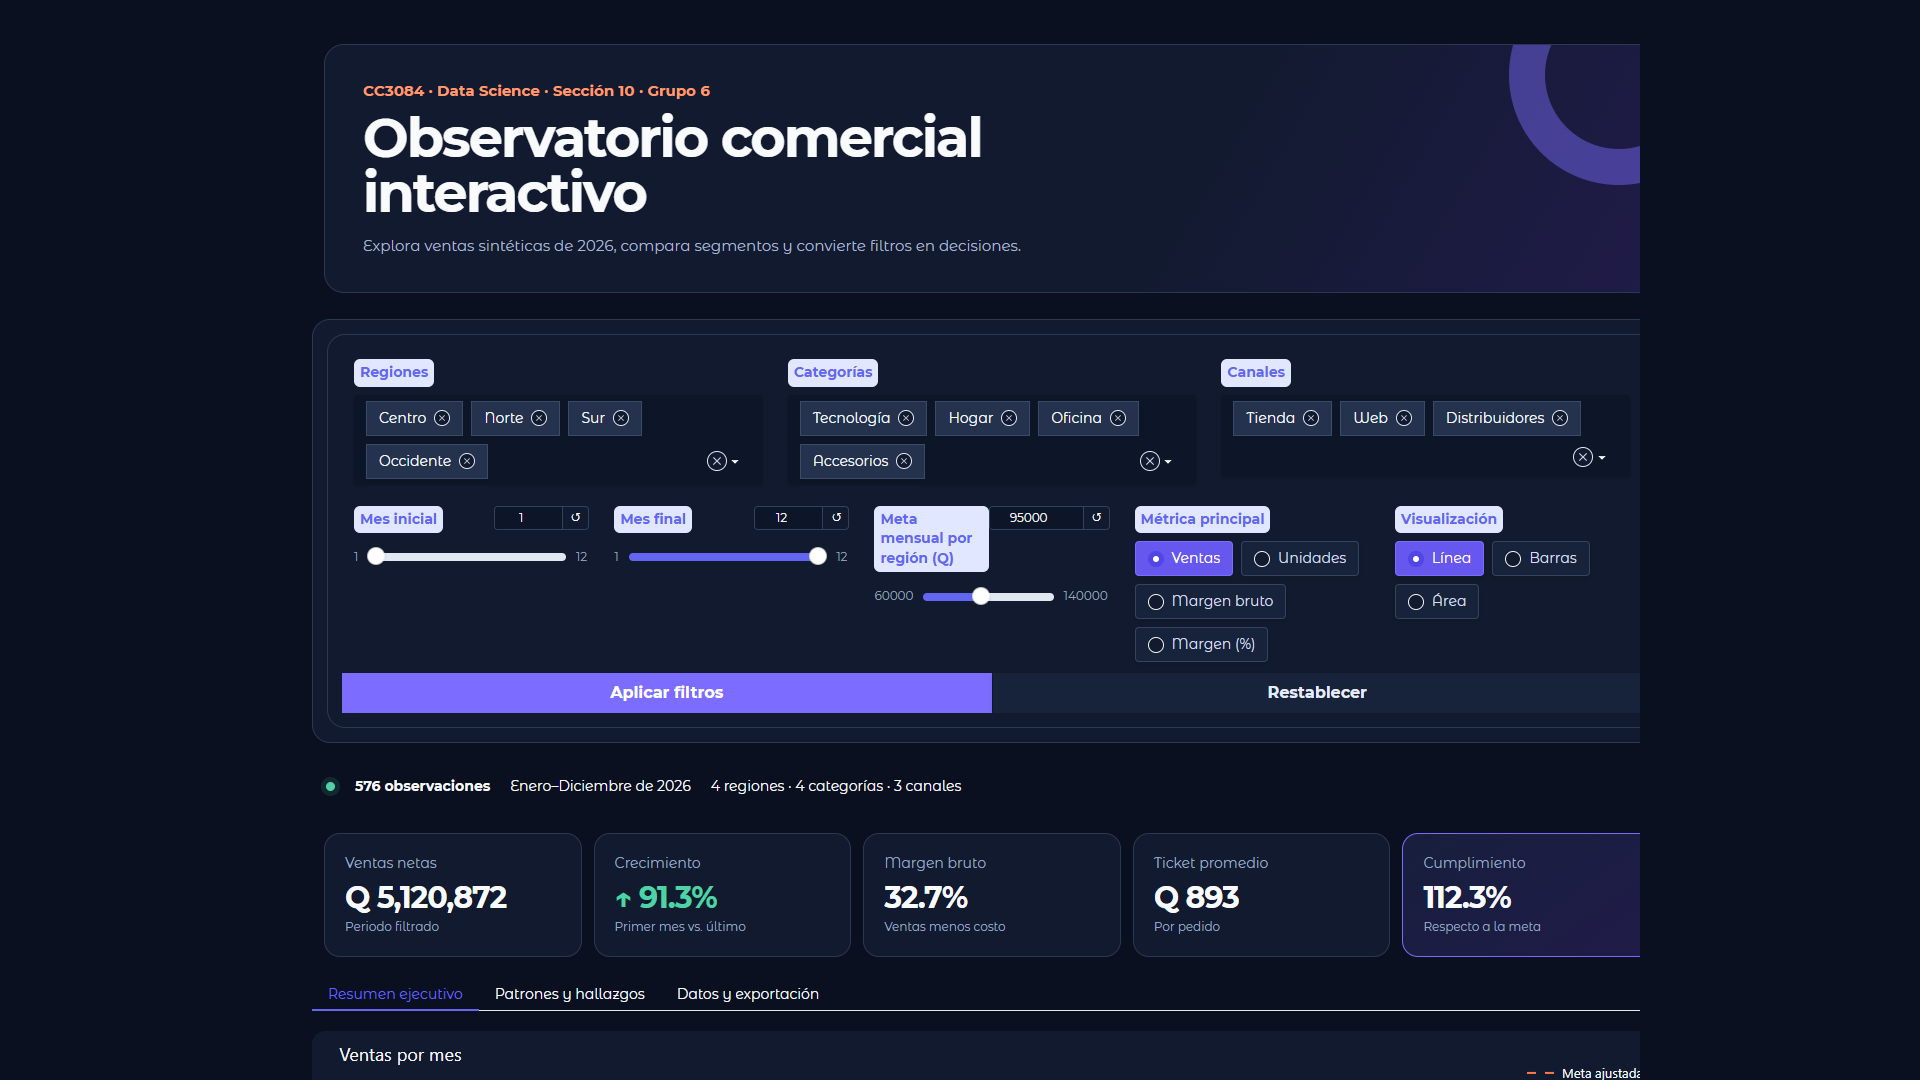
\includegraphics[width=\textwidth]{assets/dashboard_final.png}
\caption{Vista validada del observatorio comercial construido con Gradio 6.30.0.}
\end{figure}

\subsection{Cálculos principales}

El margen bruto porcentual se calcula como
\[
  \text{Margen bruto \%} = \frac{\sum (\text{Ventas} - \text{Costo})}{\sum \text{Ventas}} \times 100.
\]

El ticket promedio se define como ventas totales divididas entre pedidos. El crecimiento compara el primer y último mes visible. Para que la meta siga siendo interpretable al filtrar categorías o canales, se ajusta proporcionalmente a la cobertura seleccionada.

\subsection{Calidad y pruebas}

Se implementaron cuatro pruebas automáticas: cobertura completa del dataset, exactitud del filtrado, contrato de ocho salidas coordinadas y creación de un CSV filtrado. Adicionalmente, se verificó la aplicación en un navegador real a 1920 x 1080, se comprobó el cambio de métrica y la navegación por pestañas, y se confirmó la ausencia de errores en consola.

\section{Diseño visual y accesibilidad}

Gradio ofrece temas predefinidos y un motor de variables visuales; los temas pueden extenderse y el CSS puede suministrarse al lanzar la aplicación \cite{gradiothemes}. La documentación advierte que selectores acoplados al DOM interno pueden cambiar entre versiones, por lo que conviene utilizar clases propias y selectores estables \cite{gradiocss}.

En la aplicación se adoptaron las siguientes decisiones:

\begin{itemize}
  \item una paleta oscura consistente, independiente de la preferencia del navegador;
  \item contraste alto para texto, estados seleccionados y controles;
  \item grids responsivos con \texttt{minmax(0, 1fr)} para eliminar desbordamientos;
  \item etiquetas descriptivas y orden lógico de navegación;
  \item color acompañado de texto, no utilizado como único portador de significado;
  \item visualizaciones con títulos, ejes, leyendas y \textit{tooltips} claros.
\end{itemize}

\section{Seguridad y privacidad}

Compartir una aplicación vuelve accesible una superficie que procesa entradas externas. La guía oficial explica qué archivos pueden entrar en el caché y recomienda restringir \texttt{allowed\_paths}, utilizar \texttt{blocked\_paths} y limitar el tamaño de archivos subidos \cite{gradiofiles}.

\begin{warningbox}[title=Lista mínima antes de publicar]
\begin{itemize}
  \item No incluir claves, contraseñas o tokens en el repositorio.
  \item Validar entradas y no convertir texto del usuario directamente en una ruta local.
  \item Mantener \texttt{allowed\_paths} lo más reducido posible.
  \item Establecer \texttt{max\_file\_size} cuando existan cargas de archivos.
  \item Añadir autenticación si los datos o resultados no son públicos.
  \item Ejecutar con una cuenta de sistema con permisos mínimos.
  \item Registrar errores sin exponer trazas o secretos al usuario final.
\end{itemize}
\end{warningbox}

Los enlaces temporales creados con \texttt{share=True} son públicos; no deben considerarse un control de acceso. La aplicación continúa ejecutándose en la computadora local y el enlace actúa como túnel mientras el proceso está activo \cite{grariosharing}.

\section{Rendimiento y operación}

El rendimiento depende de la operación conectada a cada evento. Filtrar cientos de filas requiere pocos recursos; ejecutar un modelo generativo grande puede necesitar GPU y serialización cuidadosa. La documentación de colas propone ajustar concurrencia por evento y compartir colas cuando varias funciones compiten por el mismo recurso \cite{gradioqueue}.

Buenas prácticas operativas:

\begin{enumerate}
  \item cargar modelos y datos estáticos una sola vez, fuera del callback;
  \item aplicar caché a resultados deterministas costosos;
  \item limitar concurrencia según mediciones, no por intuición;
  \item paginar o resumir tablas grandes antes de enviarlas al navegador;
  \item fijar versiones en \texttt{requirements.txt};
  \item monitorear latencia, errores, memoria y longitud de cola;
  \item separar desarrollo, pruebas y producción.
\end{enumerate}

\section{Publicación y distribución}

\subsection{Ejecución local}

La opción más segura para una exposición presencial es ejecutar localmente:

\begin{codeblock}
python -m venv .venv
.venv\Scripts\activate
python -m pip install -r requirements.txt
python app.py
\end{codeblock}

\subsection{Enlace temporal}

\texttt{python app.py --share} crea una URL pública temporal. Es útil para revisión rápida, pero depende del equipo local y no sustituye un despliegue persistente \cite{grariosharing}.

\subsection{Hugging Face Spaces}

Spaces almacena el proyecto como repositorio y reconstruye la aplicación con cada actualización. Admite visibilidad pública, protegida o privada, sujeta al plan y configuración correspondiente \cite{hfspaces}. Una app Gradio alojada también puede exponerse como endpoint para clientes programáticos.

\subsection{Infraestructura propia}

Cuando existen requisitos específicos de red, observabilidad o autenticación, Gradio puede ejecutarse en infraestructura propia y montarse junto a FastAPI. En ese escenario deben definirse proxy inverso, TLS, límites de recursos, escalado, almacenamiento temporal y estrategia de actualización.

\section{Criterios de selección}

\begin{tabularx}{\textwidth}{X c c c}
\toprule
Escenario & Gradio & Framework analítico & Frontend a medida \\
\midrule
Demo de modelo de IA & \textbf{Muy adecuado} & Adecuado & Costoso para iniciar \\
Prototipo de función Python & \textbf{Muy adecuado} & Adecuado & Costoso para iniciar \\
Dashboard interno mediano & Adecuado & \textbf{Muy adecuado} & Adecuado \\
Portal empresarial complejo & Posible con evaluación & Adecuado & \textbf{Muy adecuado} \\
Identidad visual estricta & Limitado a moderado & Moderado & \textbf{Muy adecuado} \\
Entrega en pocas horas & \textbf{Muy adecuado} & Adecuado & Poco adecuado \\
\bottomrule
\end{tabularx}

La tabla no representa una regla absoluta. La experiencia del equipo, el alojamiento disponible y el tipo de usuario pueden cambiar la decisión. La recomendación es construir un prototipo pequeño y medir requisitos reales antes de comprometer una arquitectura de producción.

\section{Conclusiones}

Gradio reduce de forma notable el trabajo necesario para convertir lógica de Python en una aplicación interactiva. Su propuesta sigue alineada con el problema descrito en el trabajo original: permitir que colaboradores y usuarios de dominio prueben sistemas computacionales sin instalar el entorno del desarrollador.

La investigación muestra que su simplicidad inicial no elimina responsabilidades de ingeniería. Una aplicación pública requiere decisiones sobre estado, cola, autenticación, archivos, recursos y observabilidad. Asimismo, un buen dashboard necesita jerarquía visual, indicadores interpretables y controles que respondan a preguntas reales.

La aplicación del grupo demuestra un punto intermedio útil: conserva la rapidez de Gradio, pero incorpora segmentación multidimensional, cálculos coordinados, narrativa automática, exportación y pruebas. Por tanto, Gradio se recomienda para demos de IA, prototipos de datos, docencia y herramientas internas; para productos empresariales complejos debe compararse con frameworks analíticos o una solución web a medida.

\appendix
\section{Estructura entregada}

\begin{tabularx}{\textwidth}{>{\ttfamily\small\raggedright\arraybackslash}p{4.7cm} X}
\toprule
Archivo & Propósito \\
\midrule
app.py & Aplicación Gradio y generación del dataset sintético. \\
requirements.txt & Versiones y dependencias del proyecto. \\
tests/test\_app.py & Pruebas de datos, filtros, salidas y exportación. \\
presentacion\_\allowbreak gradio.html & Presentación interactiva autocontenida. \\
INVESTIGACION.md & Síntesis en Markdown y guion de exposición. \\
informe\_\allowbreak gradio.tex & Fuente LaTeX de este documento. \\
informe\_\allowbreak gradio.pdf & Informe compilado para entrega. \\
\bottomrule
\end{tabularx}

\section{Comandos de instalación y ejecución}

\begin{codeblock}
cd "C:\Users\Daniel Barillas\Desktop\Gradio_Data"
py -m venv .venv
.venv\Scripts\Activate.ps1
python -m pip install -r requirements.txt
python app.py
\end{codeblock}

Para ejecutar las pruebas:

\begin{codeblock}
python -m unittest discover -s tests -v
\end{codeblock}

\begin{thebibliography}{99}

\bibitem{abid2019gradio}
A. Abid, A. Abdalla, A. Abid, D. Khan, A. Alfozan y J. Zou,
``Gradio: Hassle-Free Sharing and Testing of ML Models in the Wild'',
arXiv:1906.02569, 2019.
\url{https://arxiv.org/abs/1906.02569}

\bibitem{gradioquickstart}
Gradio, ``Quickstart'', documentación oficial.
\url{https://www.gradio.app/guides/quickstart}

\bibitem{gradioblocks}
Gradio, ``Blocks'', referencia oficial.
\url{https://www.gradio.app/docs/gradio/blocks}

\bibitem{gradioqueue}
Gradio, ``Queuing'', guía oficial.
\url{https://www.gradio.app/guides/queuing}

\bibitem{gradiostate}
Gradio, ``State in Blocks'', guía oficial.
\url{https://www.gradio.app/main/guides/state-in-blocks}

\bibitem{gradiothemes}
Gradio, ``Theming Guide'', documentación oficial.
\url{https://www.gradio.app/guides/theming-guide}

\bibitem{gradiocss}
Gradio, ``Custom CSS and JS'', documentación oficial.
\url{https://www.gradio.app/guides/custom-CSS-and-JS}

\bibitem{gradiofiles}
Gradio, ``Security and File Access'', documentación oficial.
\url{https://www.gradio.app/guides/file-access}

\bibitem{grariosharing}
Gradio, ``Sharing Your App'', documentación oficial.
\url{https://www.gradio.app/guides/sharing-your-app}

\bibitem{gradiogithub}
Gradio, repositorio oficial.
\url{https://github.com/gradio-app/gradio}

\bibitem{hfspaces}
Hugging Face, ``Spaces Overview'' y ``Gradio Spaces''.
\url{https://huggingface.co/docs/hub/spaces-overview}

\bibitem{streamlitdocs}
Streamlit, documentación oficial.
\url{https://docs.streamlit.io/}

\bibitem{dashdocs}
Plotly, ``Dash Documentation''.
\url{https://dash.plotly.com/}

\bibitem{paneldocs}
HoloViz, ``Panel Documentation''.
\url{https://panel.holoviz.org/}

\bibitem{shinydocs}
Posit, ``Shiny for Python''.
\url{https://shiny.posit.co/py/}

\end{thebibliography}

\end{document}
